\subsection{Experiment 3: Missing-Value Imputation}

The AUDA analysis table is highly sparse due to substantial missing data across countries, regions, and years. For example, the United States Environmental Protection Agency (EPA) reports plastic waste generation data only at five-year intervals between 2000 and 2015. Therefore, in Experiment 3, we impute the missing values in the \texttt{YearTRC (Japan)} and \texttt{YearTRC (US)} datasets.

The experiment compares simple interpolation baselines with statistical and machine-learning imputation models. Baseline models include linear interpolation, moving average interpolation, and cubic spline interpolation, which are commonly used for filling gaps in time series. Statistical and machine learning models include ridge regression, GPR, SVR, and Theil--Sen regression.

Because both datasets have only 9 data points, each run uses only two held-out observations for testing. In this case, the denominator of \(R^2\) is very small, and modest absolute errors can produce a large negative \(R^2\). For this reason, the \(R^2\) metric is not very meaningful in this case, and we do not report it.

% results/multiple_imputation_japan/metric_table
\begin{table}[!ht]
	\centering
	\caption{\centering Imputation performance for polymer PET consumption in Japan using the \texttt{YearTRC (Japan)} dataset, averaged over 16 runs.}
	\begin{tabular}{@{}lccccc@{}}
		\toprule
		\textbf{Experiment}          & \textbf{MAE}                   & \textbf{RMSE}                  & \textbf{WAPE}       \\
		\midrule
		Linear Interpolation         & \(5.932 \times 10^4\)          & \(6.677 \times 10^4\)          & 1.59\%              \\
		Moving Average Interpolation & \(6.308 \times 10^4\)          & \(7.014 \times 10^4\)          & 1.69\%              \\
		\textbf{Cubic Spline Interpolation} & \(\mathbf{5.517 \times 10^4}\) & \(\mathbf{6.028 \times 10^4}\) & \(\mathbf{1.48}\)\% \\
		Theil-Sen Regression         & \(7.746 \times 10^4\)          & \(9.079 \times 10^4\)          & 2.08\%              \\
		Ridge Regression             & \(8.096 \times 10^4\)          & \(8.623 \times 10^4\)          & 2.17\%              \\
		GPR                          & \(7.172 \times 10^4\)          & \(8.148 \times 10^4\)          & 1.92\%              \\
		SVR                          & \(5.923 \times 10^4\)          & \(6.377 \times 10^4\)          & 1.59\%              \\
		\hline
	\end{tabular}
	\label{tab:imputation_japan_trc}
\end{table}

% results/multiple_imputation_united_states/metric_table
\begin{table}[!ht]
	\centering
	\caption{\centering Imputation performance for artificially masked total resin consumption in the United States using the \texttt{YearTRC (United States)} dataset, averaged over 16 runs with test \(n=2\) per run.}
	\begin{tabular}{@{}lccccc@{}}
		\toprule
		\textbf{Experiment}            & \textbf{MAE}                   & \textbf{RMSE}                  & \textbf{WAPE}       \\
		\midrule
		Linear Interpolation           & \(1.749 \times 10^5\)          & \(1.962 \times 10^5\)          & 1.19\%              \\
		Moving Average Interpolation   & \(3.054 \times 10^5\)          & \(3.229 \times 10^5\)          & 2.06\%              \\
		Cubic Spline Interpolation     & \(2.335 \times 10^5\)          & \(2.623 \times 10^5\)          & 1.59\%              \\
		\textbf{Theil--Sen Regression} & \(\mathbf{1.722 \times 10^5}\) & \(\mathbf{1.890 \times 10^5}\) & \(\mathbf{1.17}\)\% \\
		Ridge Regression               & \(1.902 \times 10^5\)          & \(2.091 \times 10^5\)          & 1.29\%              \\
		GPR                            & \(2.369 \times 10^5\)          & \(2.700 \times 10^5\)          & 1.61\%              \\
		SVR                            & \(1.802 \times 10^5\)          & \(1.999 \times 10^5\)          & 1.22\%              \\
		\hline
	\end{tabular}
	\label{tab:imputation_united_states_trc}
\end{table}

\begin{figure}[H]
	\centering

	\subfloat[\texttt{YearTRC (Japan)} with ridge regression.]{
		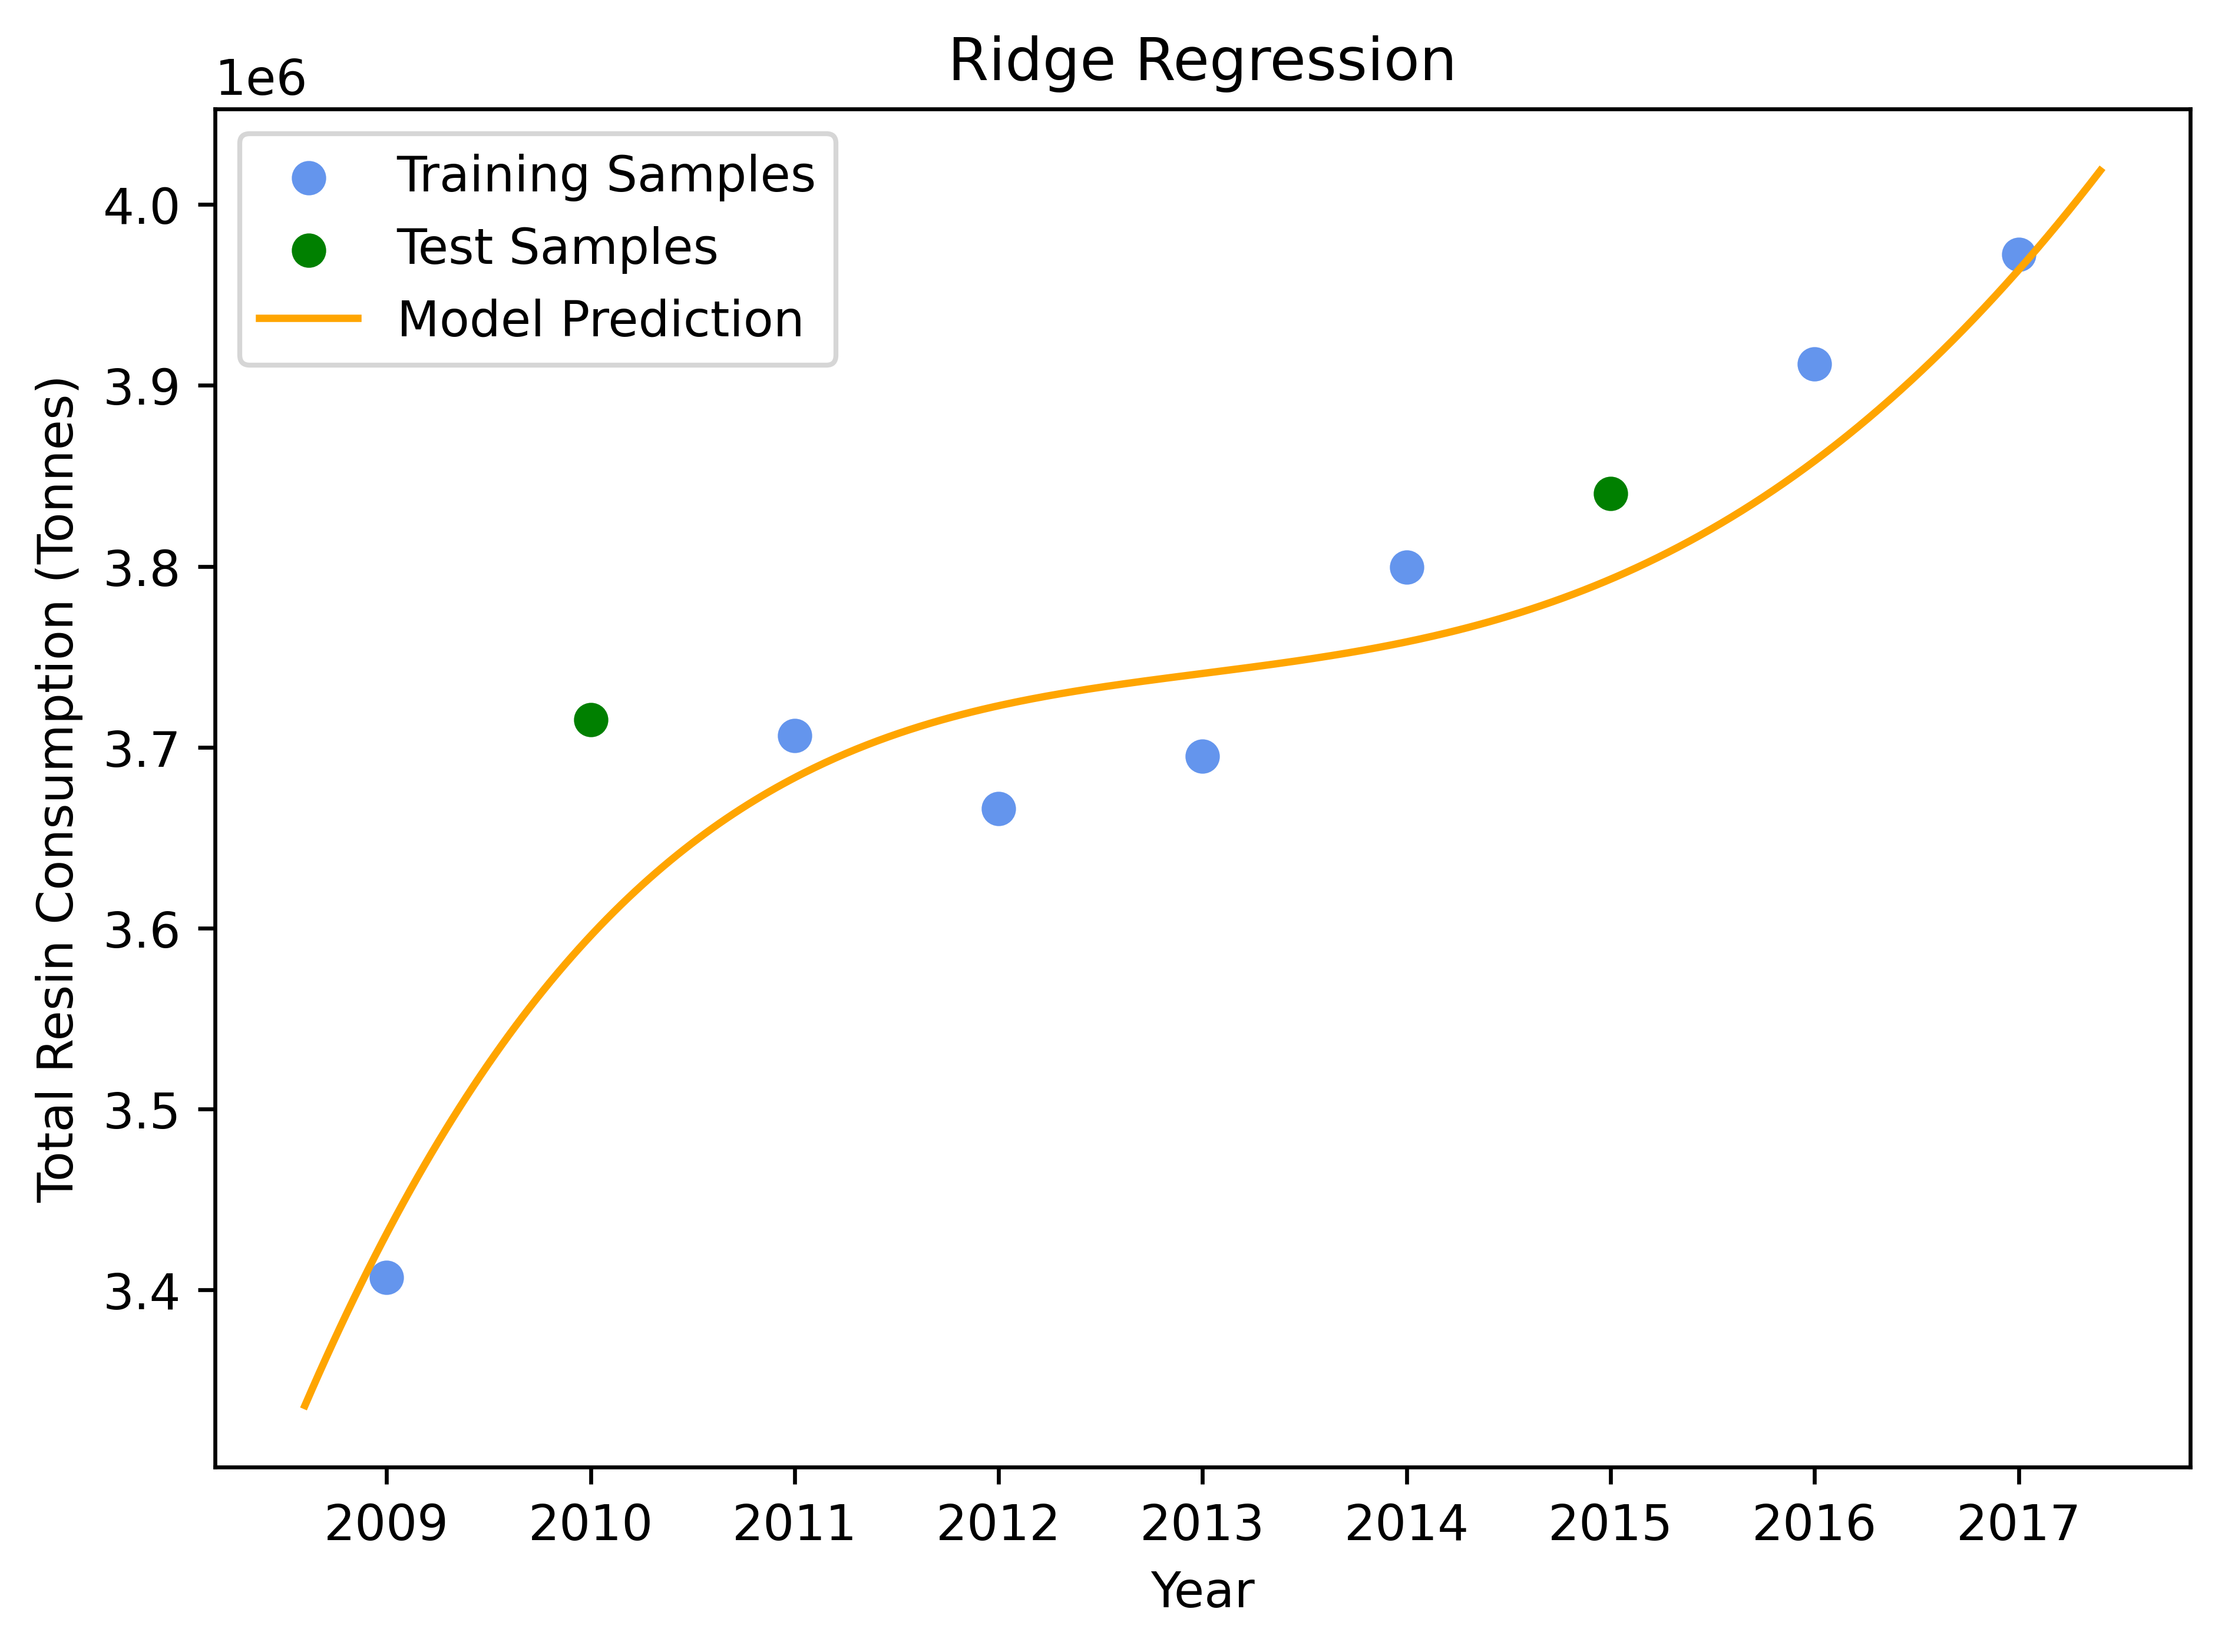
\includegraphics[width=0.45\textwidth]{figures/japan_trc_imputation_ridge_regression.png}
	}
	\subfloat[\texttt{YearTRC (Japan)} with SVR.]{
		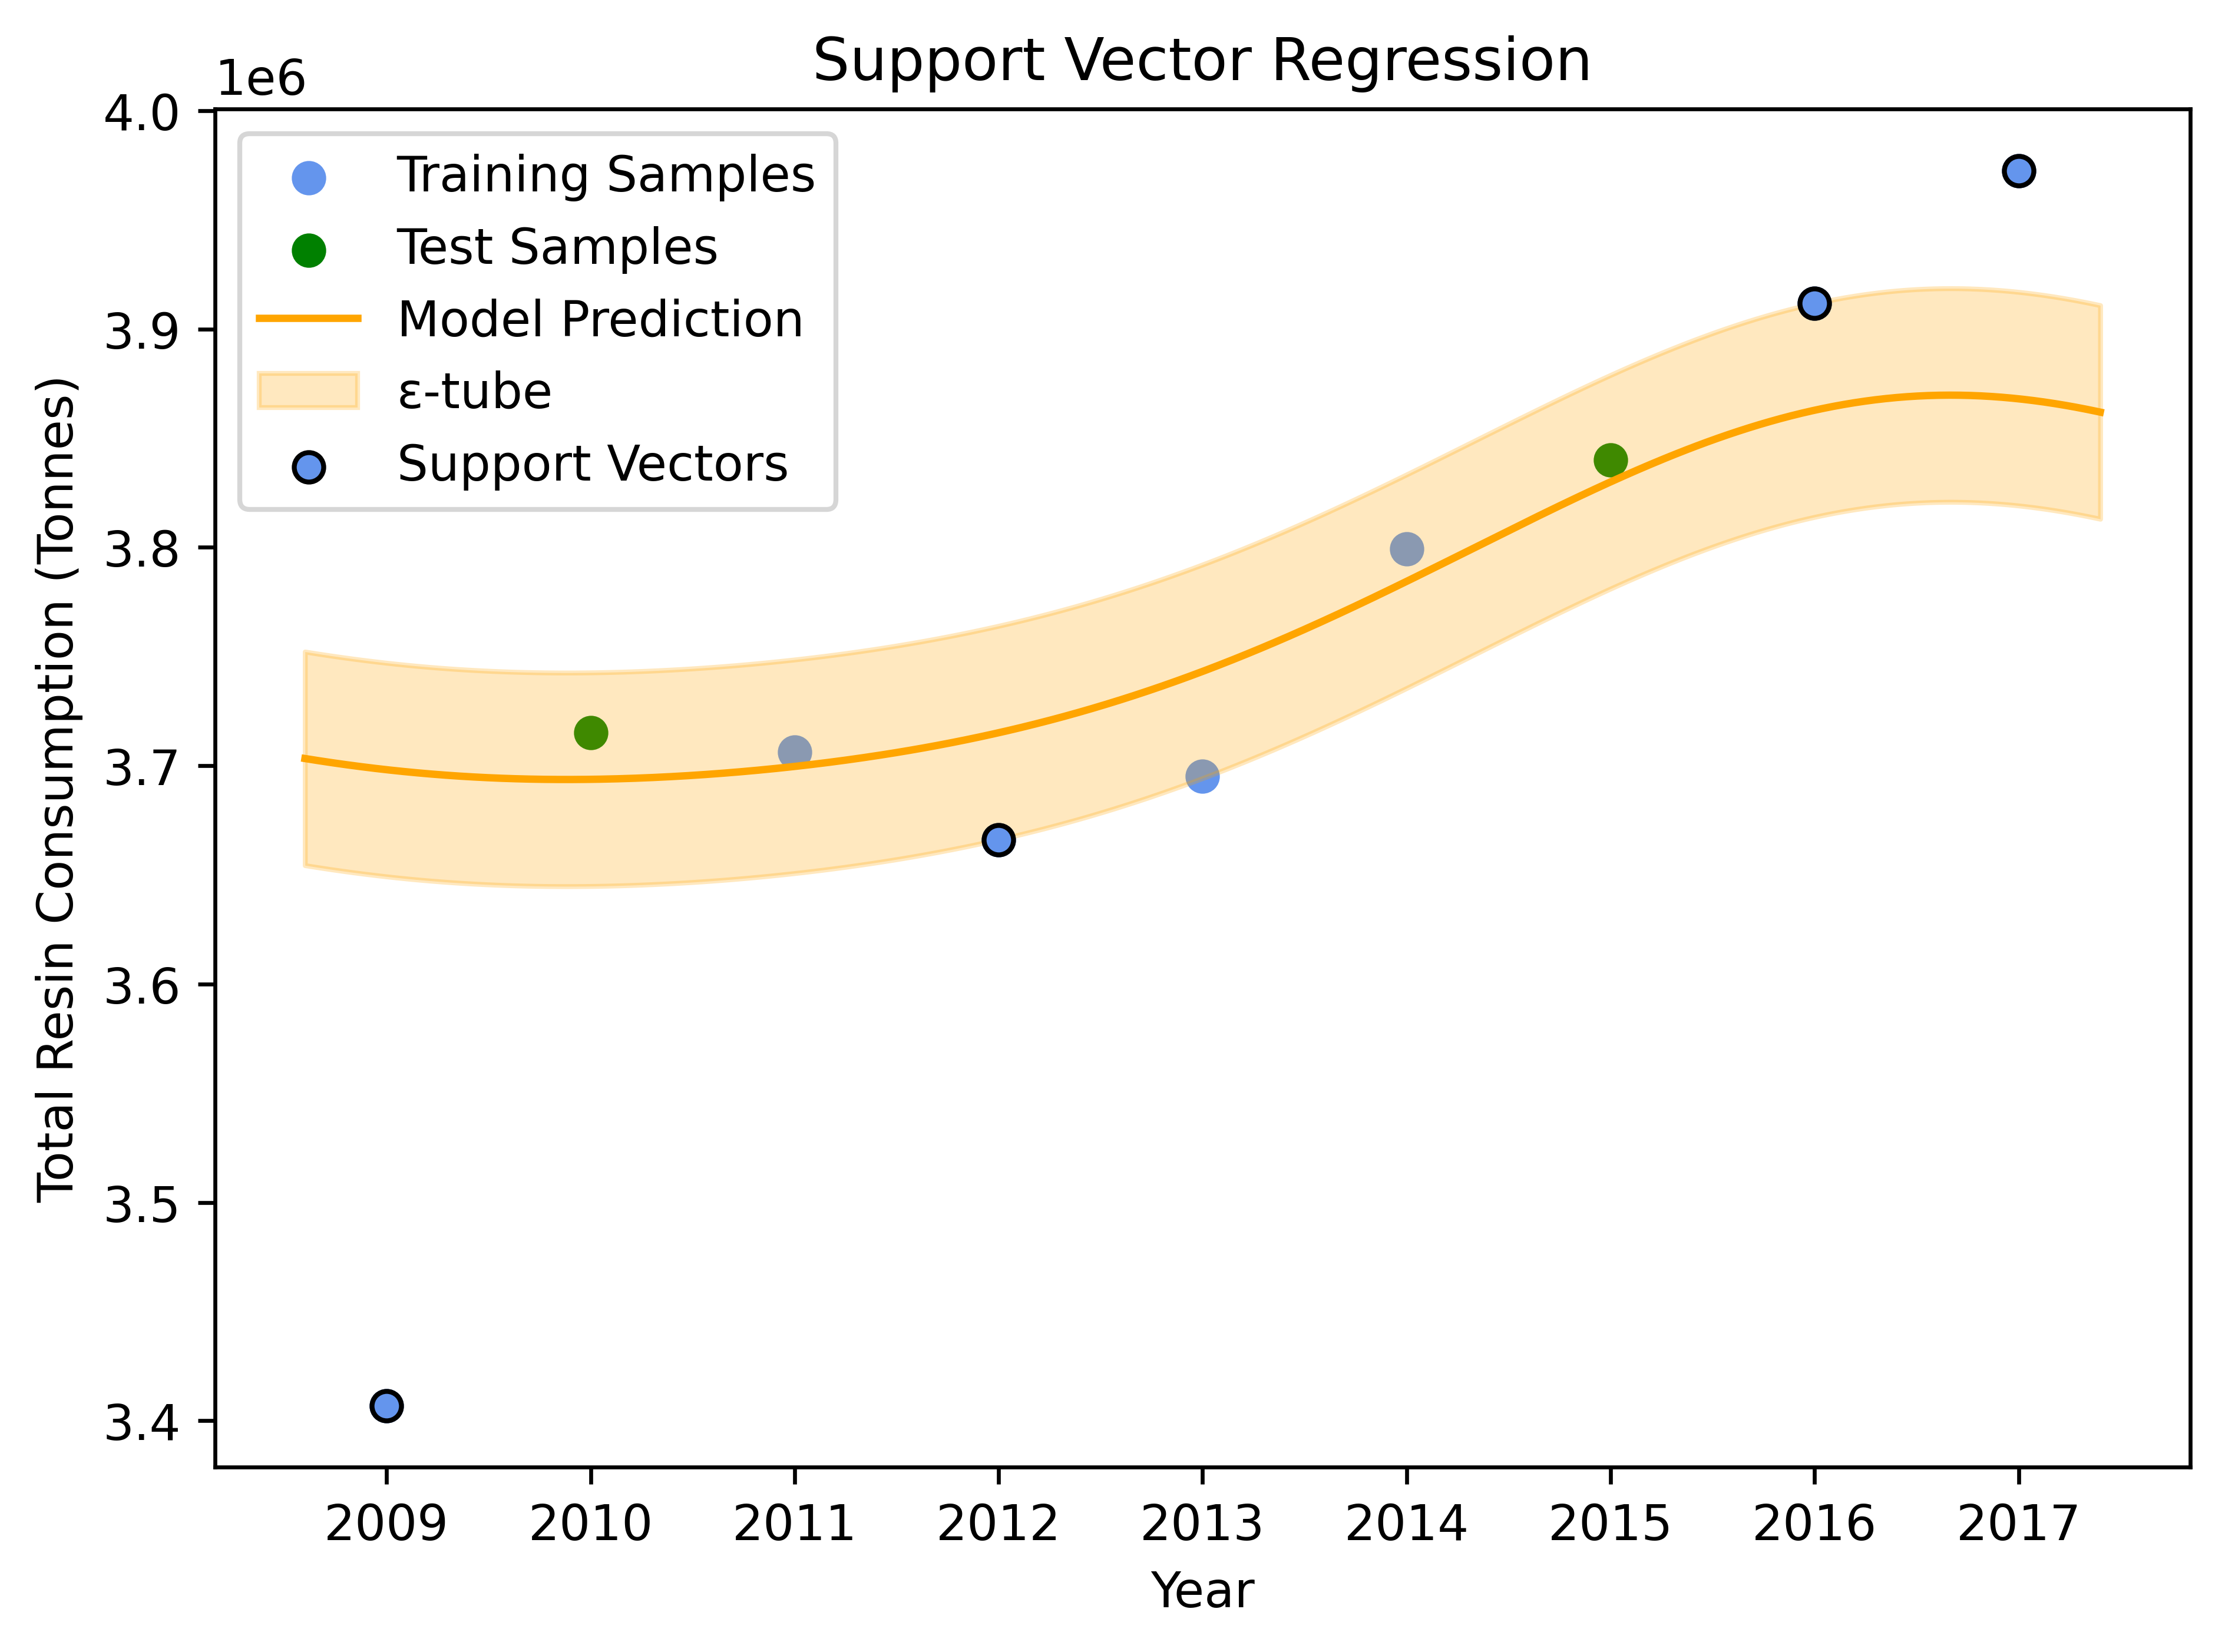
\includegraphics[width=0.45\textwidth]{figures/japan_trc_imputation_svr.png}
	}

	\vspace{0.5cm}

	\subfloat[\texttt{YearTRC (United States)} with GPR.]{
		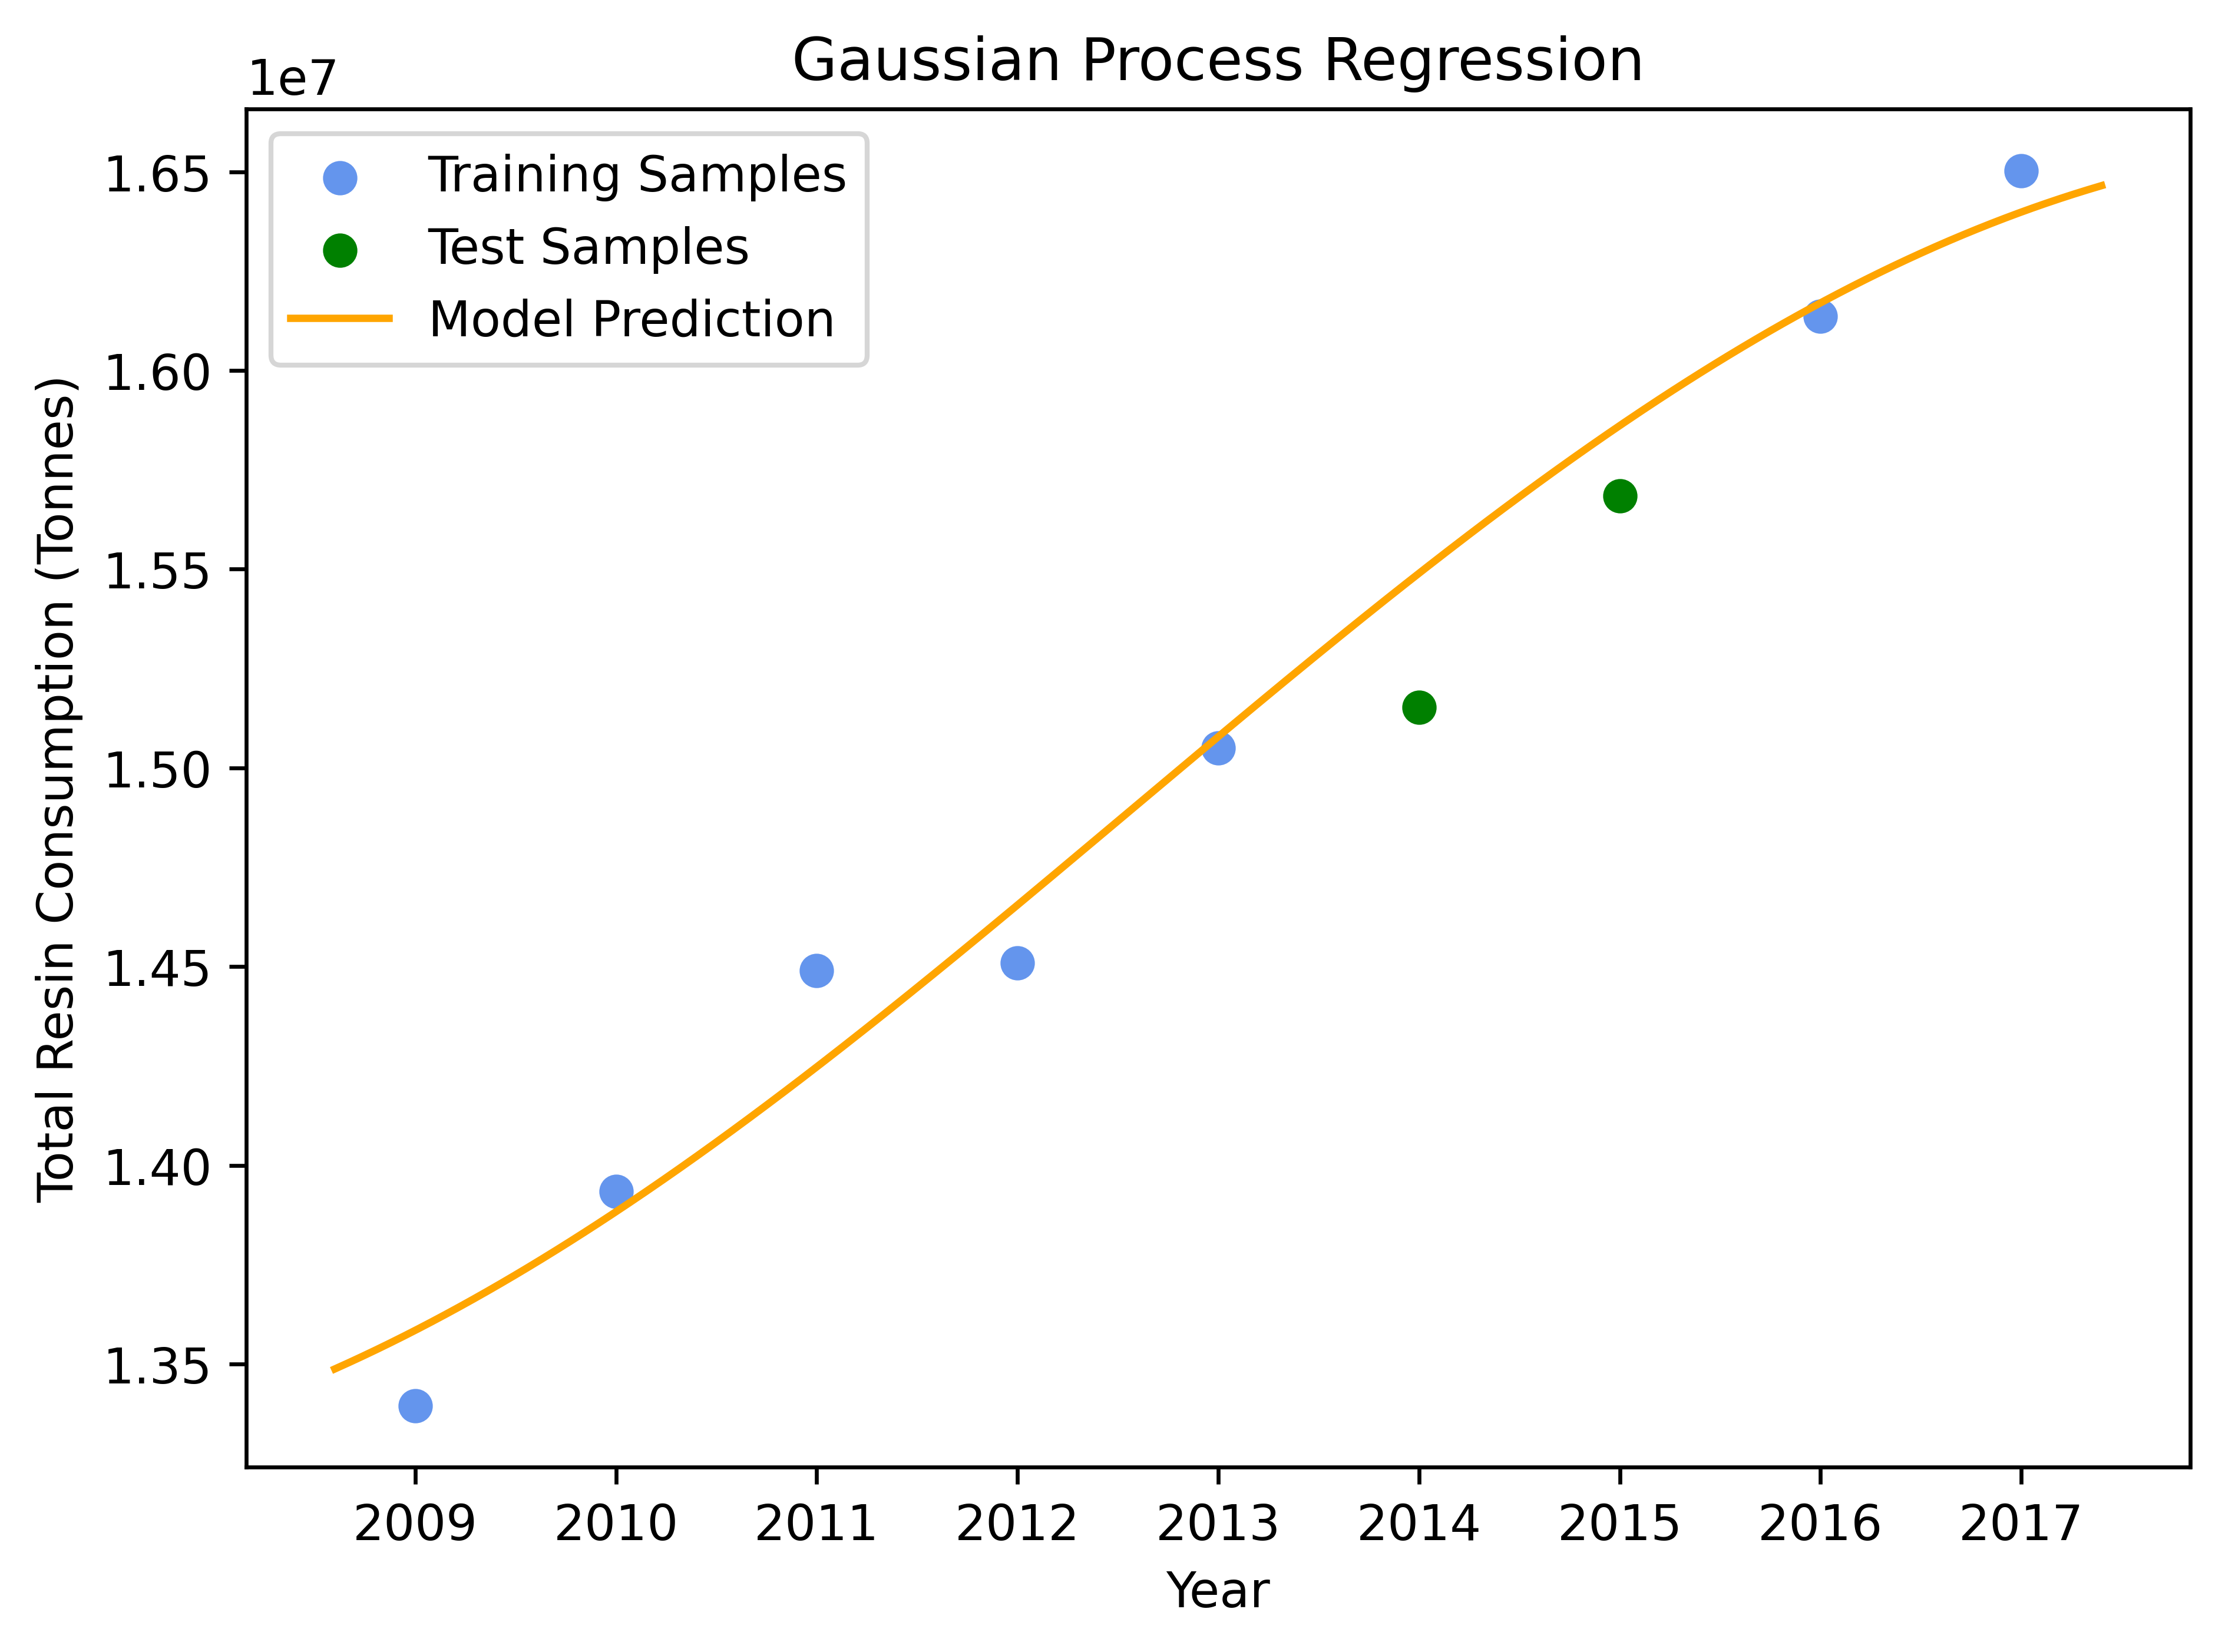
\includegraphics[width=0.45\textwidth]{figures/united_states_trc_imputation_gpr.png}
	}
	\hfill
	\subfloat[\texttt{YearTRC (United States)} with SVR.]{
		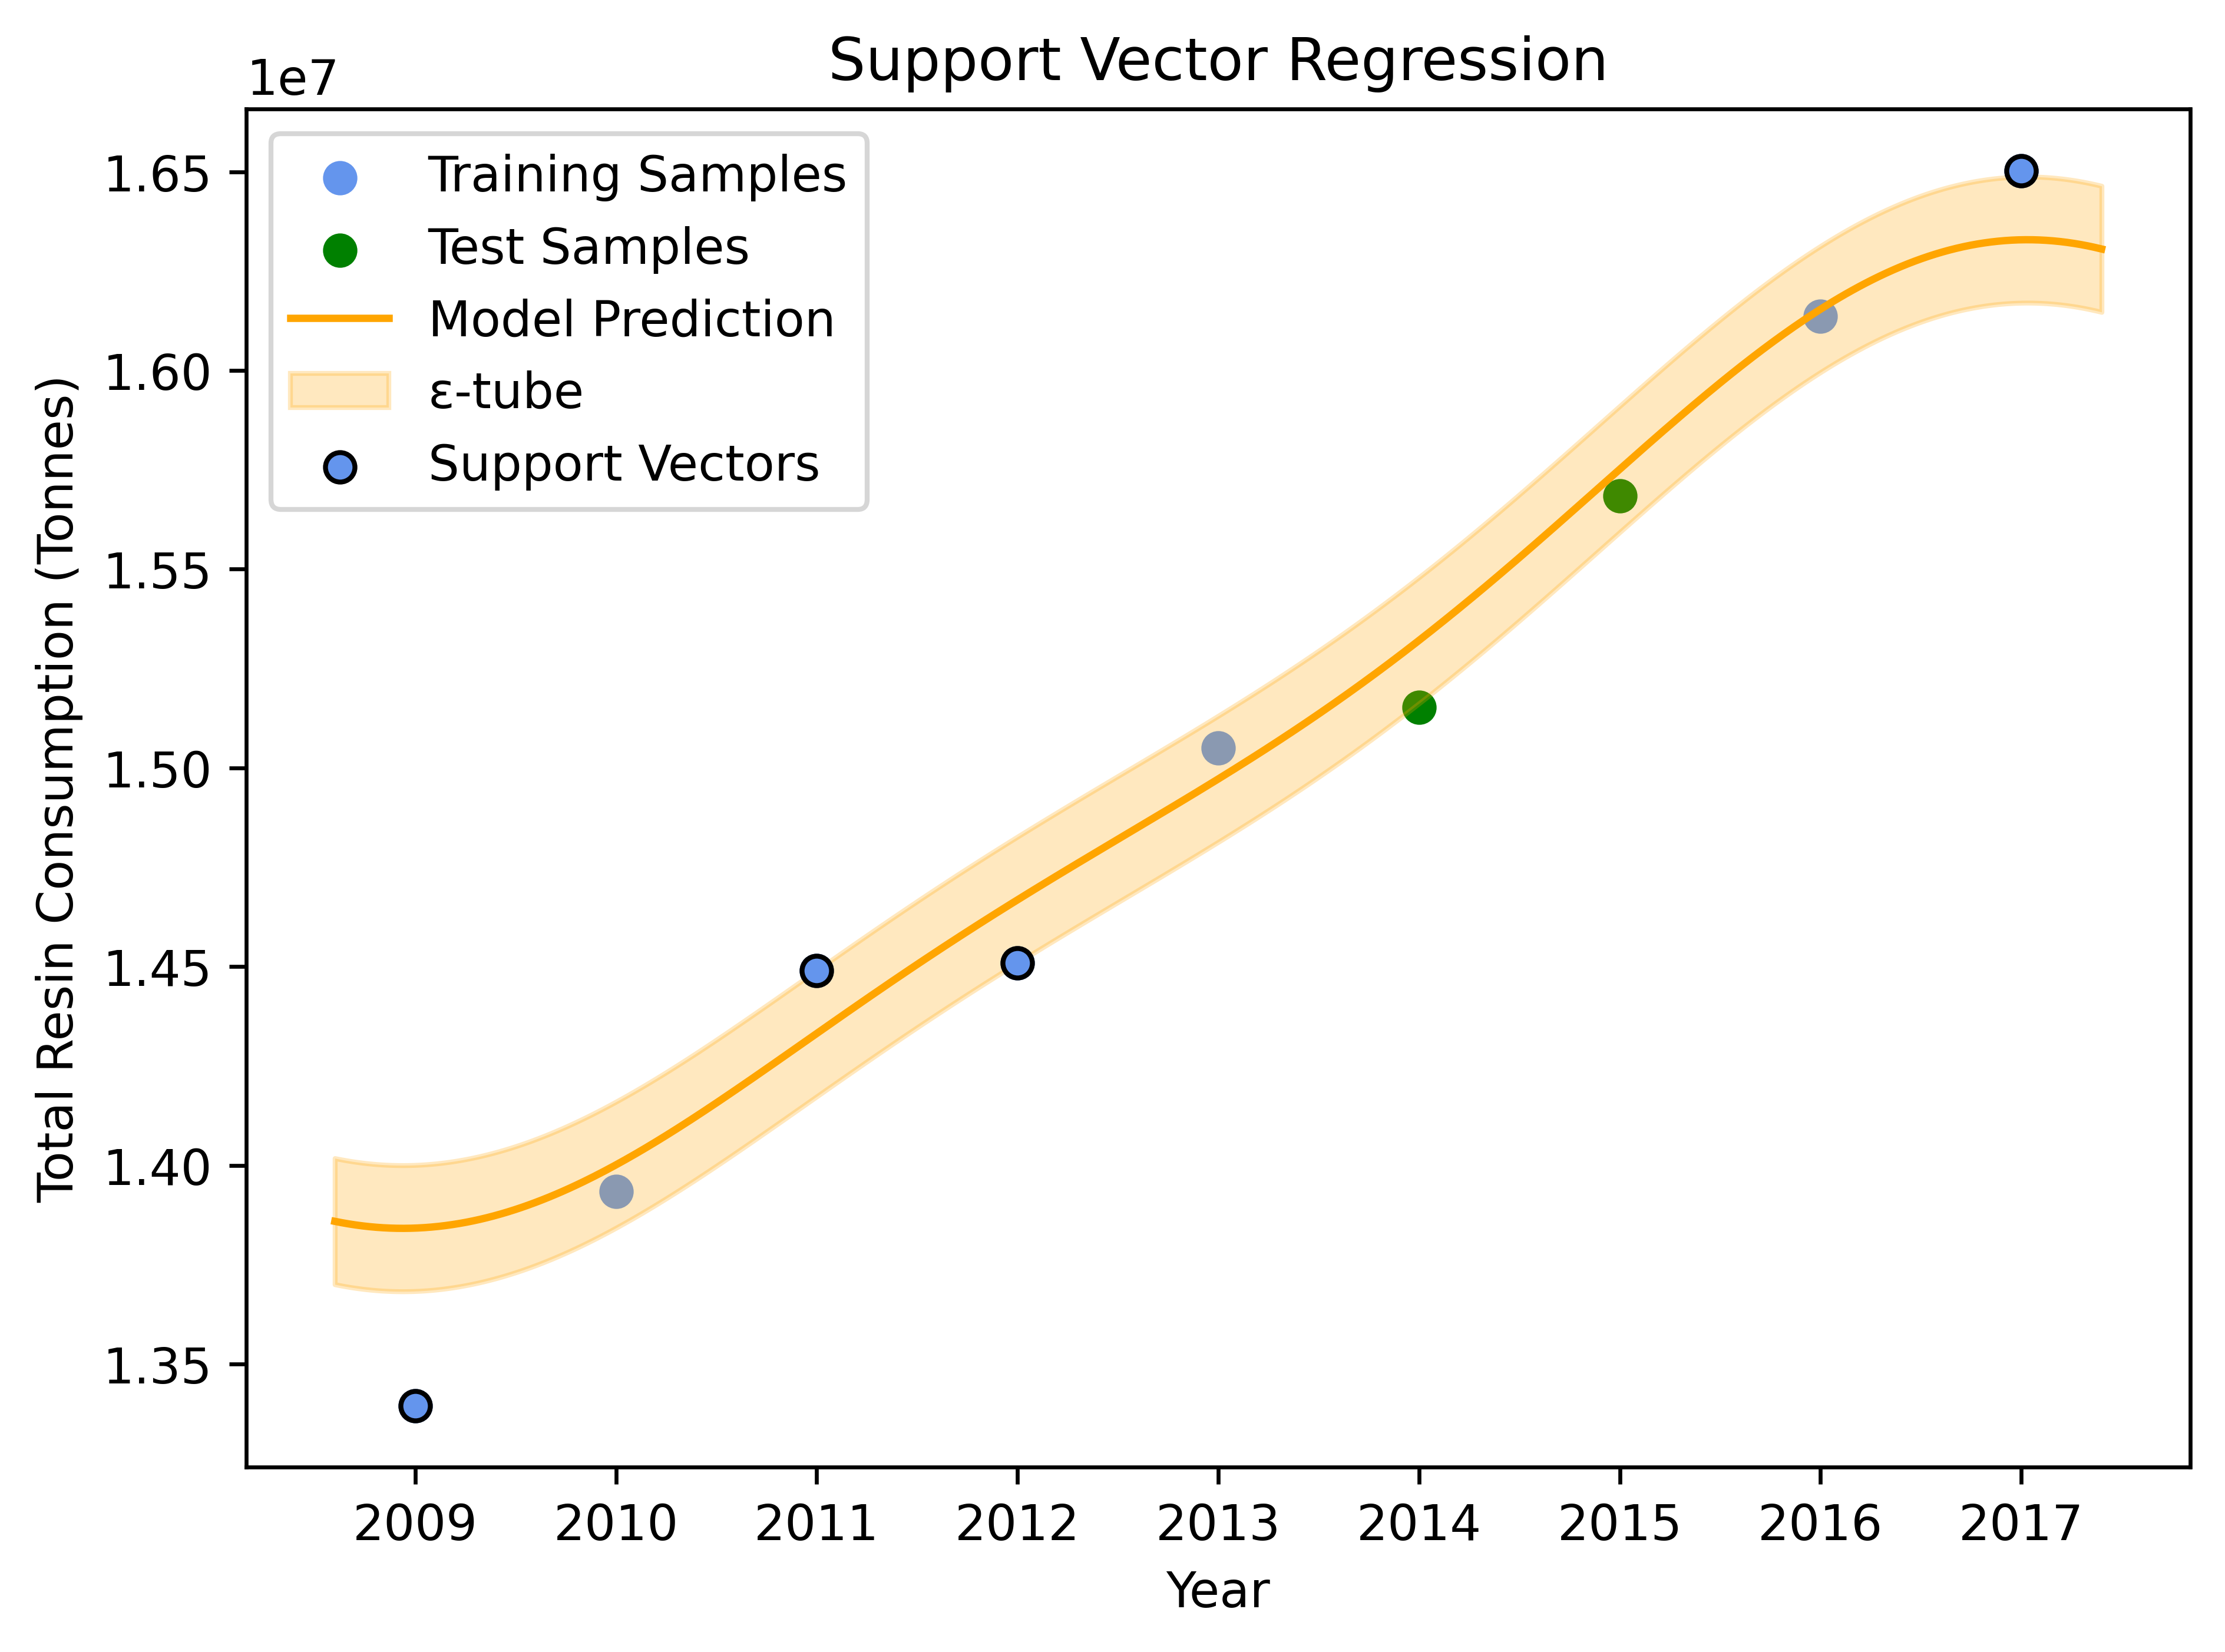
\includegraphics[width=0.45\textwidth]{figures/united_states_trc_imputation_svr.png}
	}

	\caption{Imputation plots for the \texttt{YearTRC} dataset: ridge regression and SVR for Japan, and GPR and SVR for the United States.}

	\label{fig:imputation_plots}
\end{figure}


Table~\ref{tab:imputation_japan_trc} shows that SVR performs best on the \texttt{YearTRC (Japan)} imputation task, with the lowest MAE, RMSE, and WAPE among the evaluated methods. Its WAPE is 1.36\%, compared with 1.48\% for cubic spline interpolation and 1.59\% for linear interpolation.

Table~\ref{tab:imputation_united_states_trc} shows a slightly different pattern for the \texttt{YearTRC (US)} task. SVR still gives the best overall result, with a WAPE of 1.08\%, while Theil--Sen regression and linear interpolation are also competitive at 1.17\% and 1.19\%, respectively. These results indicate that the United States series can be imputed accurately by both flexible machine learning models and smoother trend-based methods.

Figure~\ref{fig:imputation_plots} shows representative fitted trajectories from the imputation experiments. The \texttt{YearTRC (Japan)} series exhibits a more nonlinear trend than the \texttt{YearTRC (US)} series. The results for both tasks show that SVR can handle both linear and relatively nonlinear trends well.
